\section{Date: 2026-10-11}
\noindent \textbf{Series ID: LAURD840000000000004A} 

\noindent This series is titled Unemployed Persons in West North Central Census Division and has a frequency of Annual. The units are Persons and the seasonal adjustment is Not Seasonally Adjusted.The observation start date is 1976-01-01 and the observation end date is 2025-01-01.The popularity of this series is 1. \\ 

\noindent \textbf{Series ID: LAURD870000000000005} 

\noindent This series is titled Employed Persons in West South Central Census Division and has a frequency of Monthly. The units are Persons and the seasonal adjustment is Not Seasonally Adjusted.The observation start date is 1976-01-01 and the observation end date is 2026-08-01.The popularity of this series is 1. \\ 

\subsection{Raw Regression}
\noindent Regresses the two series against each other directly. A significant result here can come just as easily from both series sharing a long-run trend as from any real relationship.

\begin{center}
\begin{tabular}{lclc}
\toprule
\textbf{Dep. Variable:}                     & value\_fred\_LAURD870000000000005 & \textbf{  R-squared:         } &     0.000   \\
\textbf{Model:}                             &                OLS                & \textbf{  Adj. R-squared:    } &    -0.021   \\
\textbf{Method:}                            &           Least Squares           & \textbf{  F-statistic:       } &  0.008385   \\
\textbf{Date:}                              &          Sun, 11 Oct 2026         & \textbf{  Prob (F-statistic):} &    0.927    \\
\textbf{Time:}                              &              16:51:42             & \textbf{  Log-Likelihood:    } &   -818.30   \\
\textbf{No. Observations:}                  &                   50              & \textbf{  AIC:               } &     1641.   \\
\textbf{Df Residuals:}                      &                   48              & \textbf{  BIC:               } &     1644.   \\
\textbf{Df Model:}                          &                    1              & \textbf{                     } &             \\
\textbf{Covariance Type:}                   &             nonrobust             & \textbf{                     } &             \\
\bottomrule
\end{tabular}
\begin{tabular}{lcccccc}
                                            & \textbf{coef} & \textbf{std err} & \textbf{t} & \textbf{P$> |$t$|$} & \textbf{[0.025} & \textbf{0.975]}  \\
\midrule
\textbf{const}                              &    1.445e+07  &     1.82e+06     &     7.961  &         0.000        &     1.08e+07    &     1.81e+07     \\
\textbf{value\_fred\_LAURD840000000000004A} &      -0.3451  &        3.769     &    -0.092  &         0.927        &       -7.923    &        7.232     \\
\bottomrule
\end{tabular}
\begin{tabular}{lclc}
\textbf{Omnibus:}       &  4.099 & \textbf{  Durbin-Watson:     } &    0.011  \\
\textbf{Prob(Omnibus):} &  0.129 & \textbf{  Jarque-Bera (JB):  } &    1.836  \\
\textbf{Skew:}          &  0.023 & \textbf{  Prob(JB):          } &    0.399  \\
\textbf{Kurtosis:}      &  2.062 & \textbf{  Cond. No.          } & 1.95e+06  \\
\bottomrule
\end{tabular}
%\caption{OLS Regression Results}
\end{center}

Notes: \newline
 [1] Standard Errors assume that the covariance matrix of the errors is correctly specified. \newline
 [2] The condition number is large, 1.95e+06. This might indicate that there are \newline
 strong multicollinearity or other numerical problems.

\begin{figure}
\centering
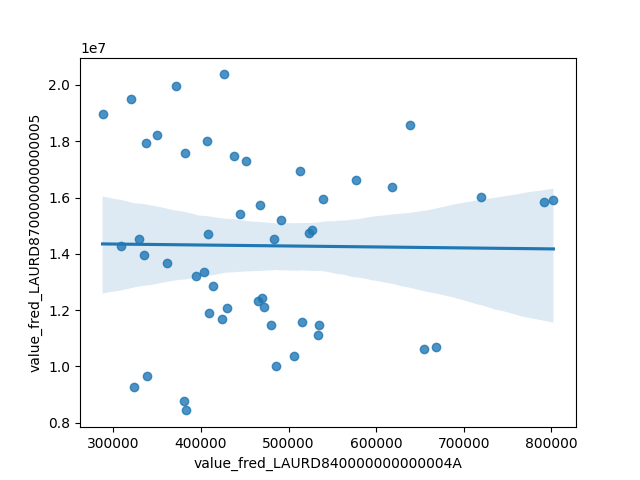
\includegraphics[scale = 0.9]{plots/plot_2026-10-11.png}
\caption{Raw Regression Plot for 2026-10-11}
\end{figure}
\newpage
\subsection{Detrended Regression}
\noindent Regresses the residuals of each series after removing its own linear time trend, so a shared trend can no longer drive the result on its own. A relationship that stays significant here is better evidence of a genuine link between the two series.

\begin{center}
\begin{tabular}{lclc}
\toprule
\textbf{Dep. Variable:}                                & value\_fred\_LAURD870000000000005\_detrended & \textbf{  R-squared:         } &     0.054   \\
\textbf{Model:}                                        &                     OLS                      & \textbf{  Adj. R-squared:    } &     0.034   \\
\textbf{Method:}                                       &                Least Squares                 & \textbf{  F-statistic:       } &     2.733   \\
\textbf{Date:}                                         &               Sun, 11 Oct 2026               & \textbf{  Prob (F-statistic):} &    0.105    \\
\textbf{Time:}                                         &                   16:51:42                   & \textbf{  Log-Likelihood:    } &   -700.71   \\
\textbf{No. Observations:}                             &                        50                    & \textbf{  AIC:               } &     1405.   \\
\textbf{Df Residuals:}                                 &                        48                    & \textbf{  BIC:               } &     1409.   \\
\textbf{Df Model:}                                     &                         1                    & \textbf{                     } &             \\
\textbf{Covariance Type:}                              &                  nonrobust                   & \textbf{                     } &             \\
\bottomrule
\end{tabular}
\begin{tabular}{lcccccc}
                                                       & \textbf{coef} & \textbf{std err} & \textbf{t} & \textbf{P$> |$t$|$} & \textbf{[0.025} & \textbf{0.975]}  \\
\midrule
\textbf{const}                                         &    1.419e-07  &     4.26e+04     &  3.33e-12  &         1.000        &    -8.57e+04    &     8.57e+04     \\
\textbf{value\_fred\_LAURD840000000000004A\_detrended} &      -0.5932  &        0.359     &    -1.653  &         0.105        &       -1.315    &        0.128     \\
\bottomrule
\end{tabular}
\begin{tabular}{lclc}
\textbf{Omnibus:}       &  1.421 & \textbf{  Durbin-Watson:     } &    0.552  \\
\textbf{Prob(Omnibus):} &  0.491 & \textbf{  Jarque-Bera (JB):  } &    0.654  \\
\textbf{Skew:}          &  0.147 & \textbf{  Prob(JB):          } &    0.721  \\
\textbf{Kurtosis:}      &  3.476 & \textbf{  Cond. No.          } & 1.19e+05  \\
\bottomrule
\end{tabular}
%\caption{OLS Regression Results}
\end{center}

Notes: \newline
 [1] Standard Errors assume that the covariance matrix of the errors is correctly specified. \newline
 [2] The condition number is large, 1.19e+05. This might indicate that there are \newline
 strong multicollinearity or other numerical problems.

\begin{figure}
\centering
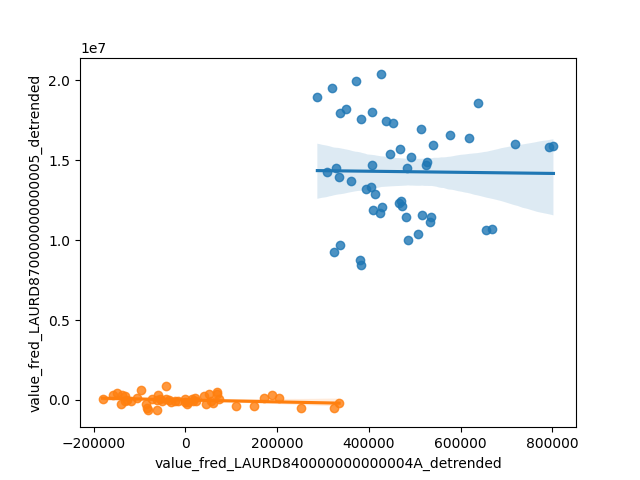
\includegraphics[scale = 0.9]{plots/plot_2026-10-11_detrended.png}
\caption{Detrended Regression Plot for 2026-10-11}
\end{figure}
\newpage
